Before diving into each measurement in detail, we'll look at the overall trends in the data collected by the MassDEP reference sensors relative to our learnAir sensors.  As we can see in Figure \ref{fig:repa_ref_measures}, there are four reference measurements taken, each with slower moving trends as well as clear transient spikes.  

We expect transient events in CO, NO2, and black carbon, the direct by-products of combustion.  As noted in the background section, these pollutants frequently vary with rapid time-scales, and their transient phenomena have been well characterized.  O3 is also known to have transient events, despite the more complicated reactions that drive its creation.  This behavior has been modeled, and studies of other cities have shown similar magnitude/duration transient behavior in measured O3 levels.  It is suspected that meteorological conditions and high NOx are to blame in rapid ozone formation, as well as large concentrations of other highly reactive VOCs. \cite{ozonehouston, houstonvoc, Trevino1999}

\begin{figure}[htb]
 	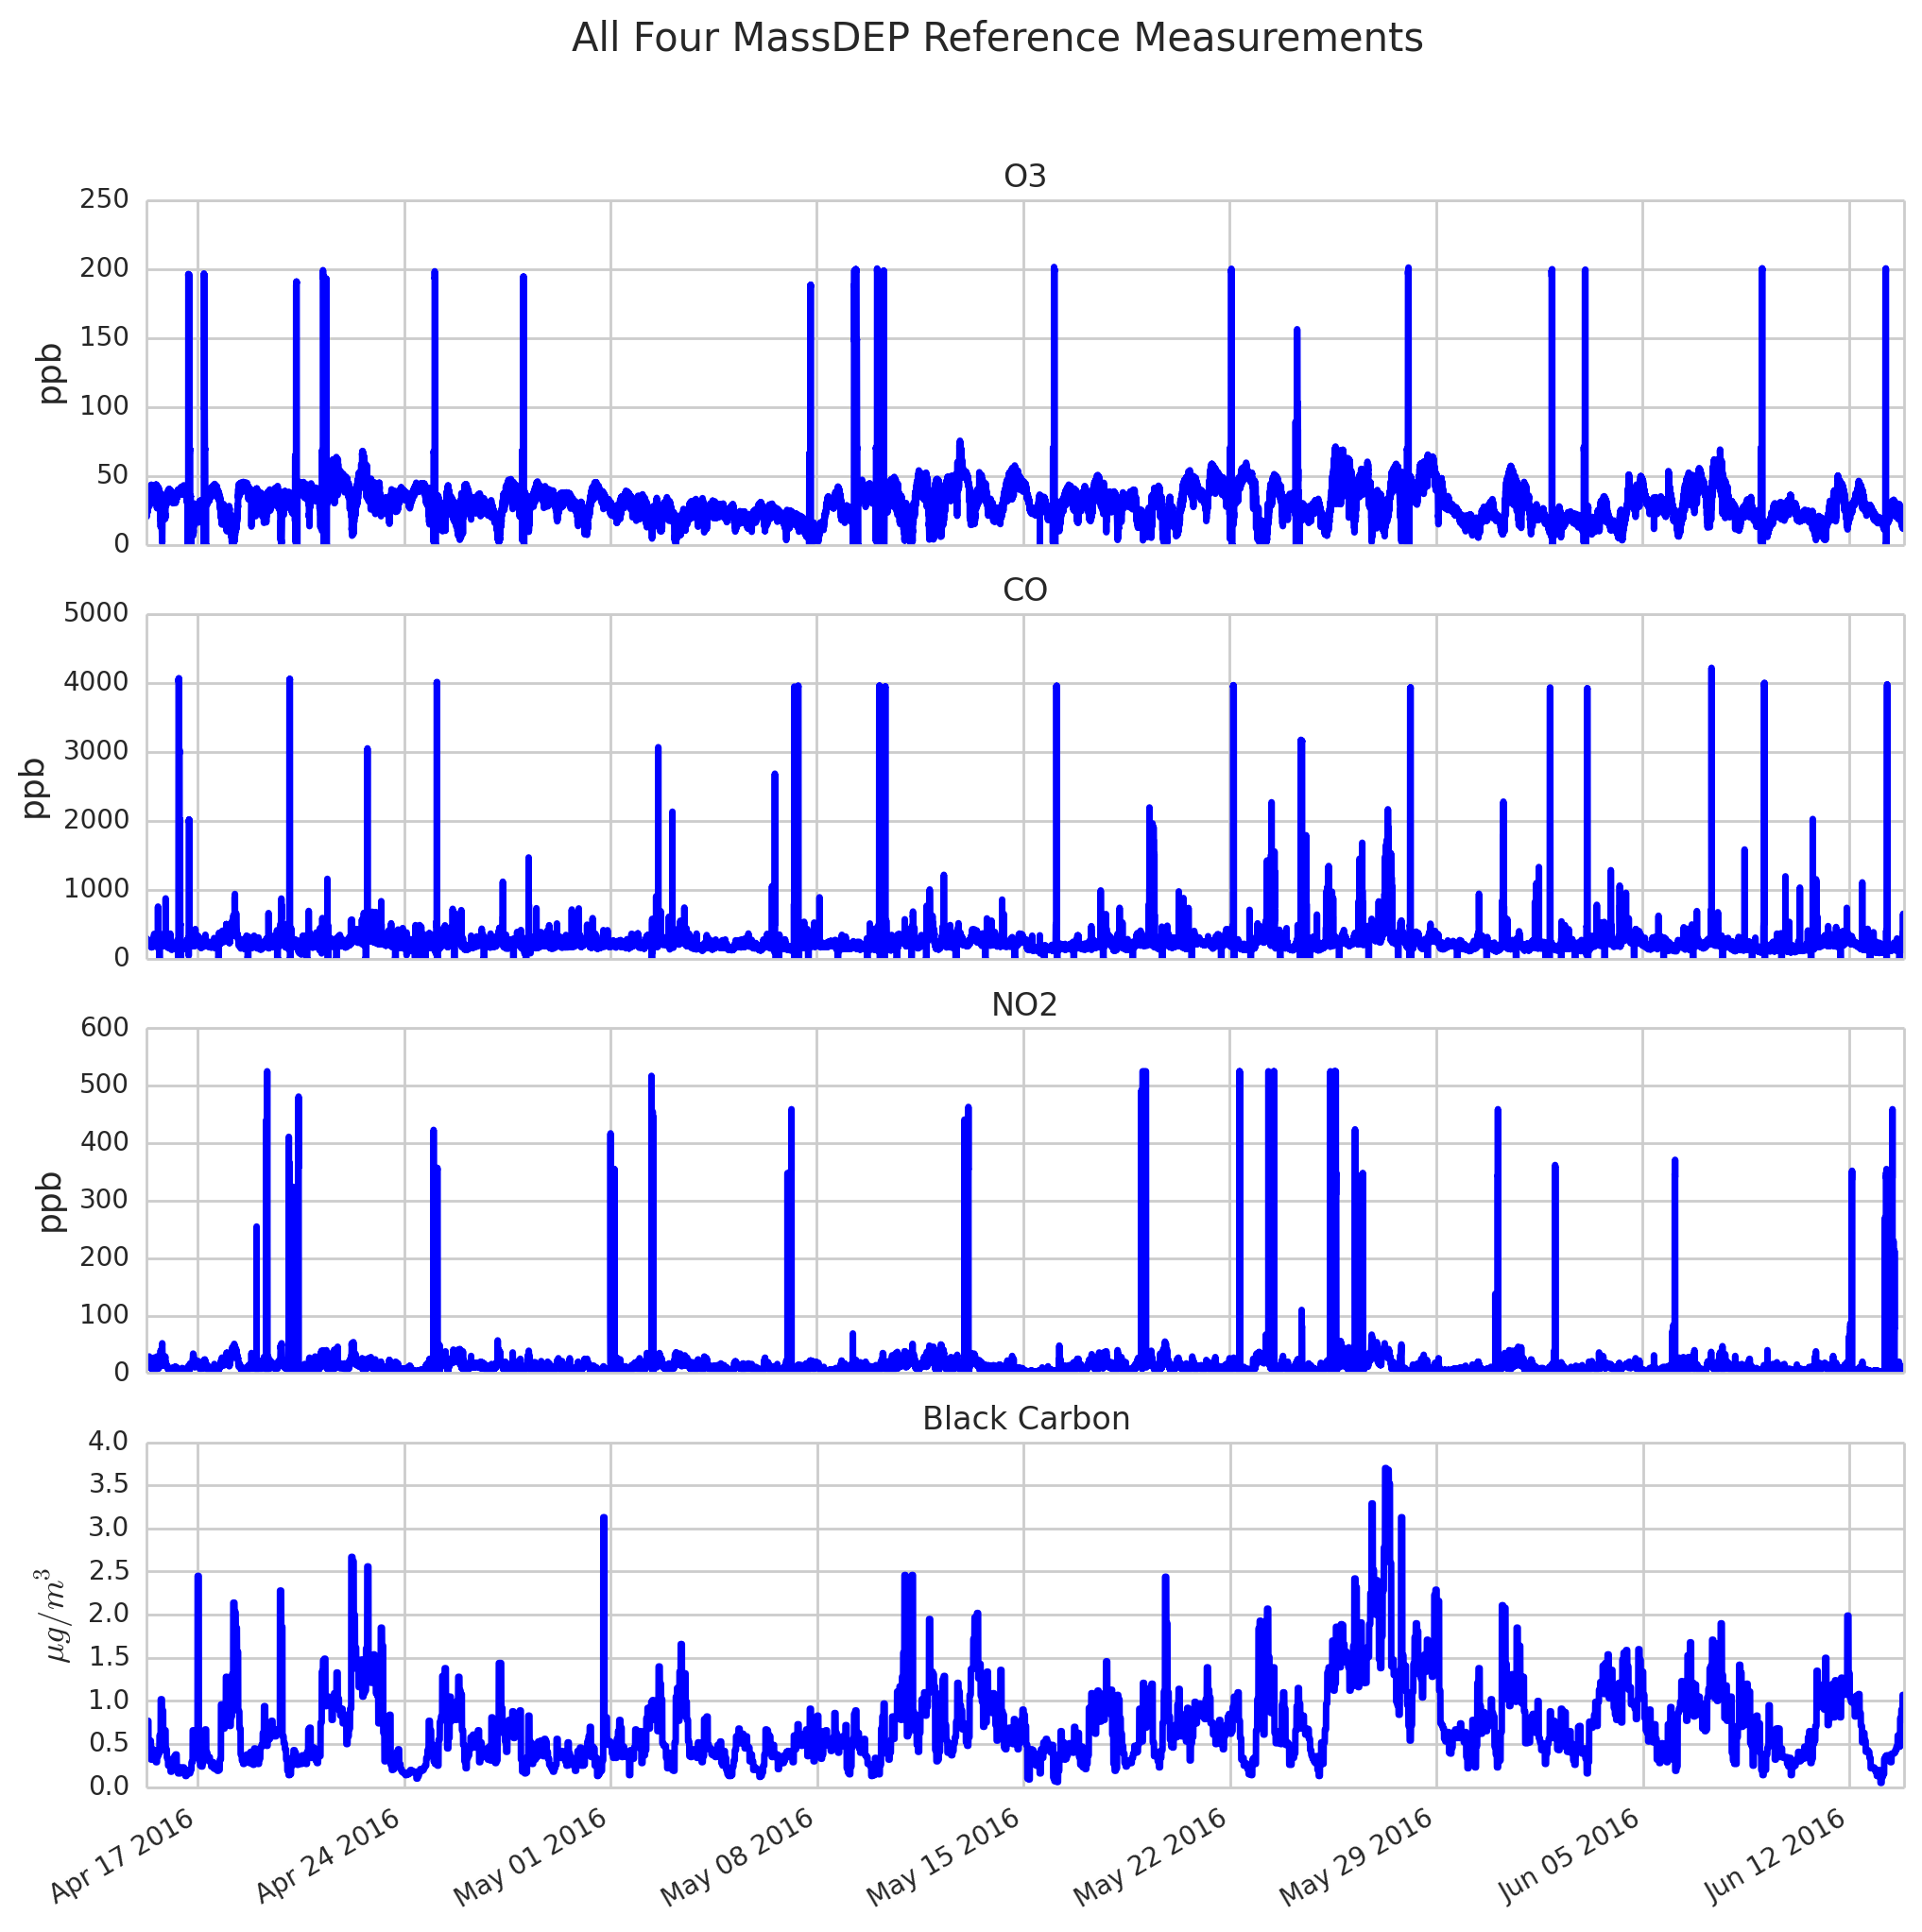
\includegraphics[width=\textwidth]{figs/epa_ref_measures}               
 	 \caption{Reference Sensors Measurements During Test Period}
  	\label{fig:epa_ref_measures}
\end{figure}

Zooming in on these transient events reveals their duration-- NO2 transients fall in the minute-duration range, while O3 and CO tend to sustain for about half an hour at a time.  Black carbon is integrated hourly, so true transient behavior cannot be observed.  

The variability of pollutant concentration as a function of temperature, wind speed, emission flow rate, emission concentration level,  and flue height (which is modeled itself on a variety of parameters) greatly affects dispersion characteristics.  The distance from roadside and height of these sensors makes it quite plausible that transient events will disperse before reaching a sensor and occur over longer time-scales. \cite{kaur2007}  The lack of clear relationships between time-of-day and these transients-- as well as the relative independence of each sensor-- is not surprising.  It does appear a subset of NO2, CO, and O3 transient events occur close in time, and likely share a causal link (as would be expected, since they are associated with the same sources-- likely heavy diesel traffic for this installation).  


\begin{marginfigure}
	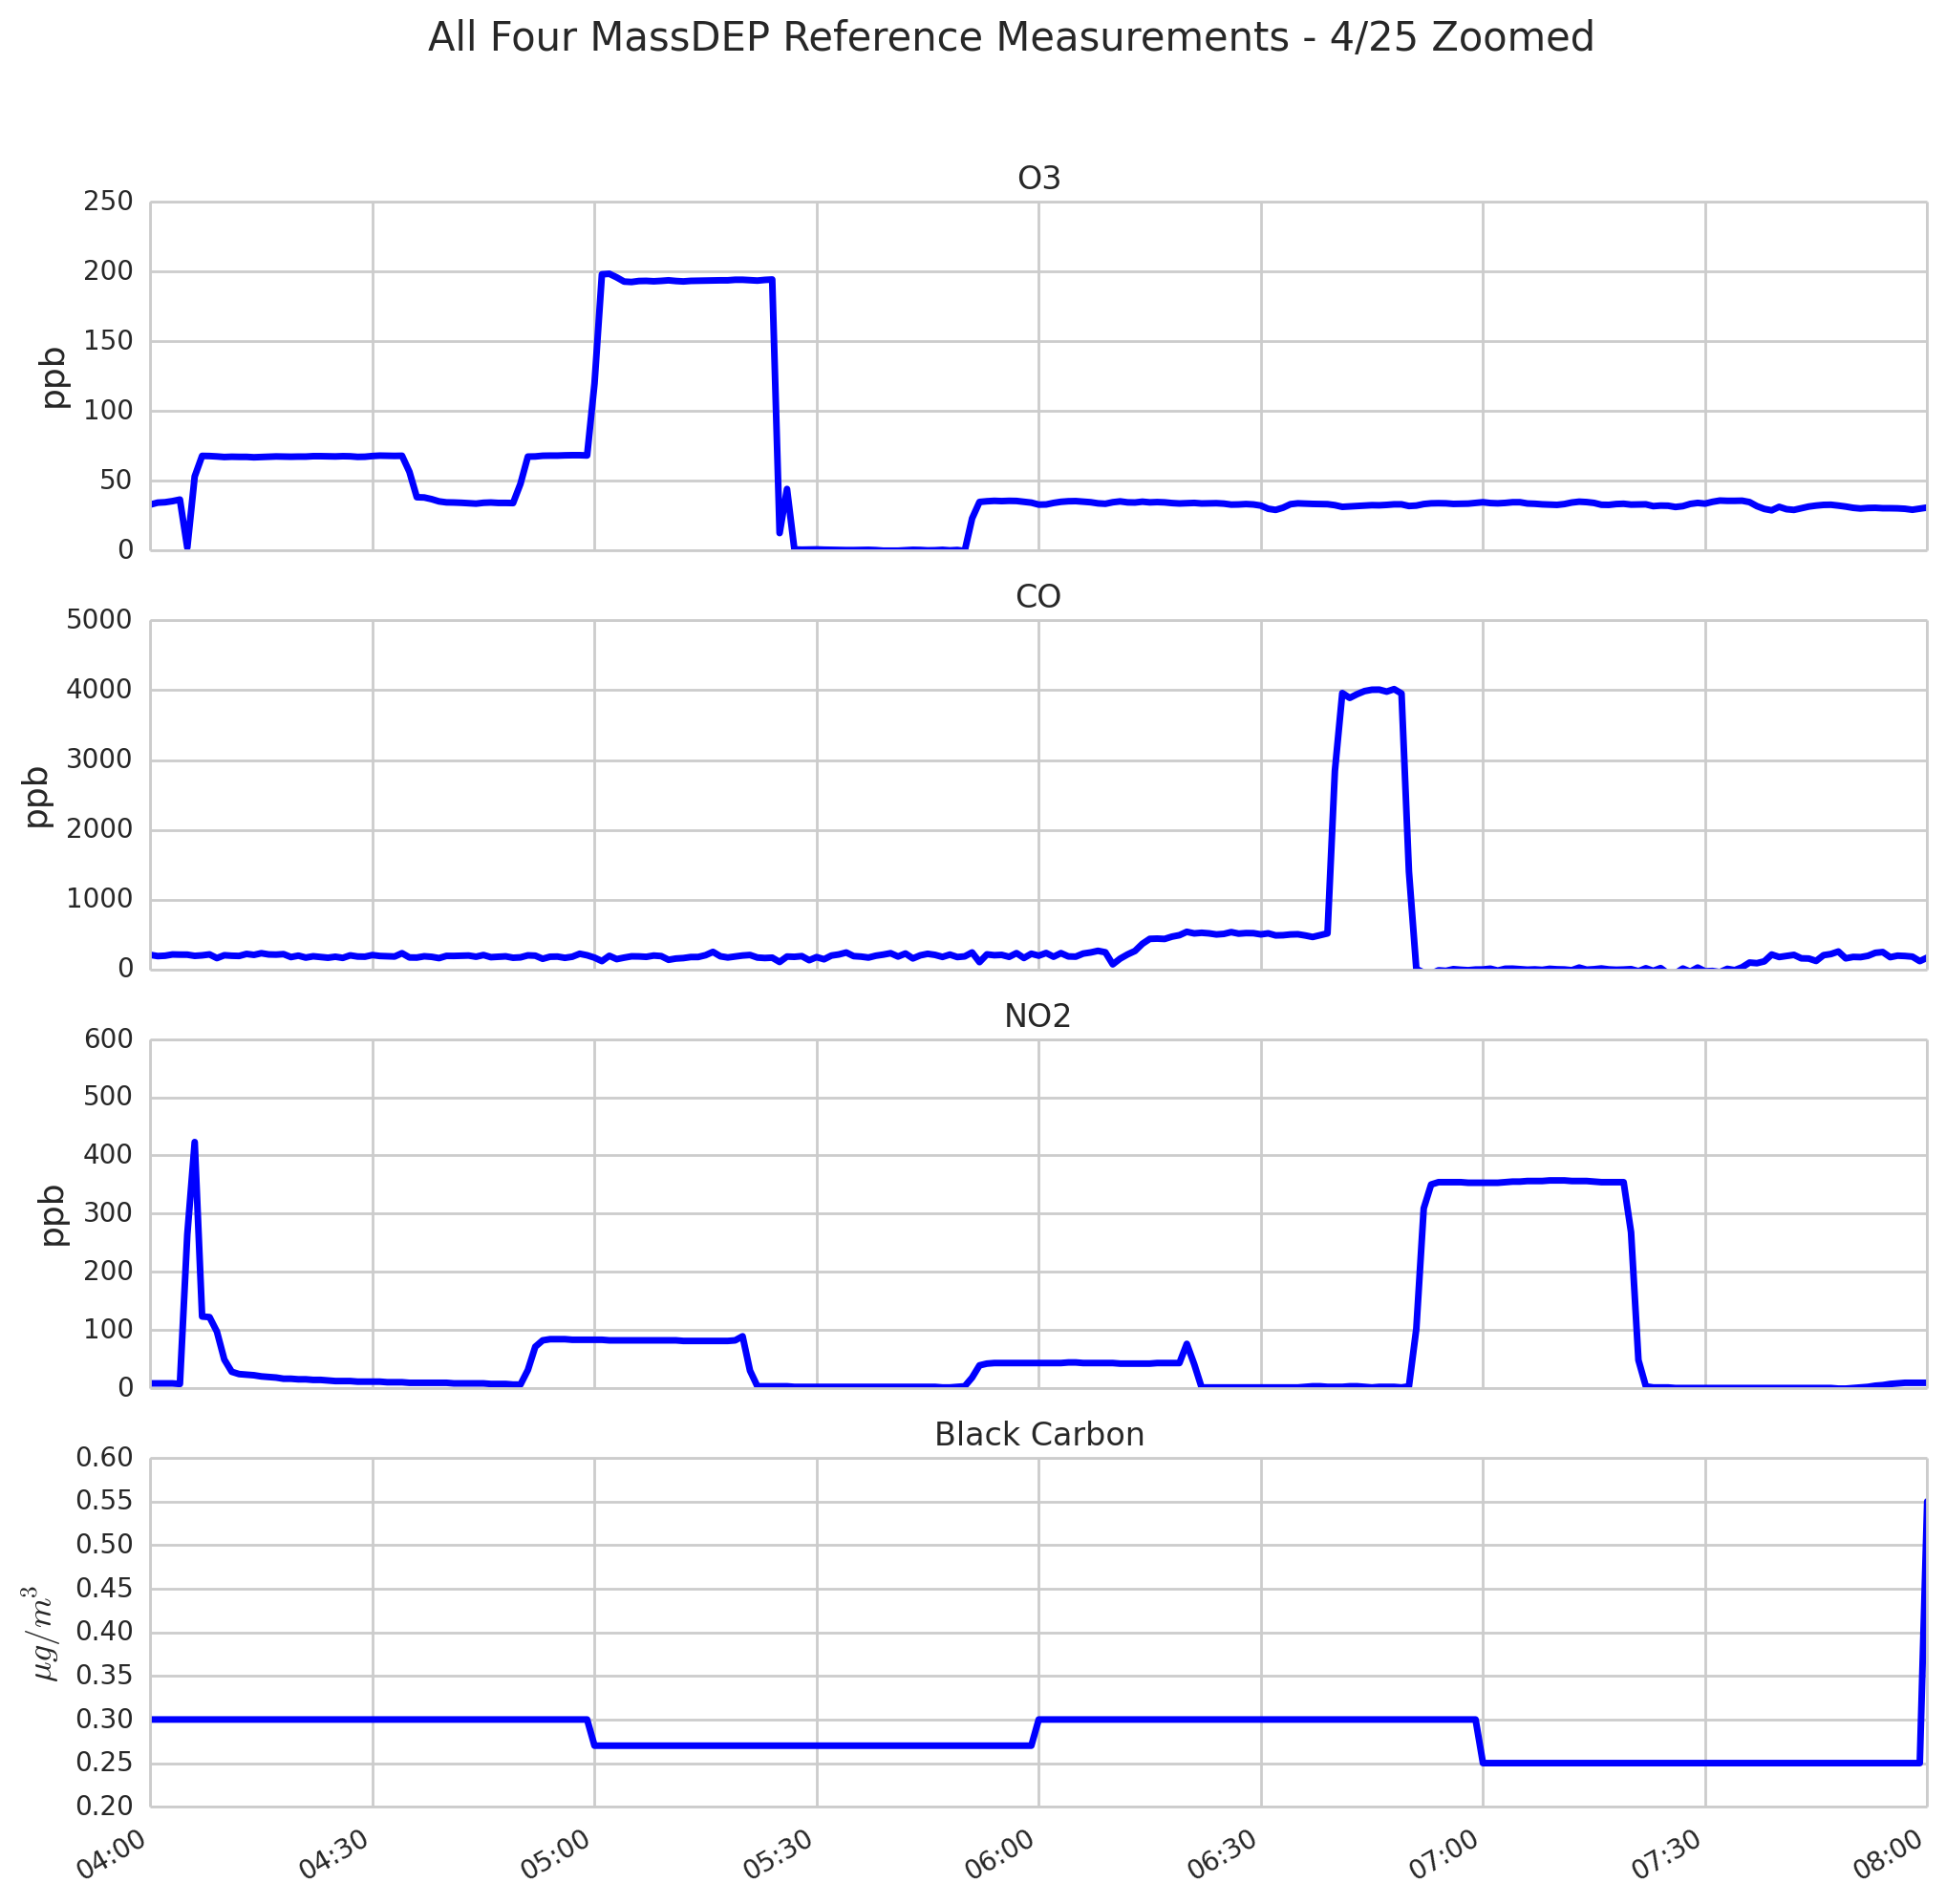
\includegraphics[width=\textwidth]{figs/epa_ref_measures_zoomed2}  
	\par
	\par
 	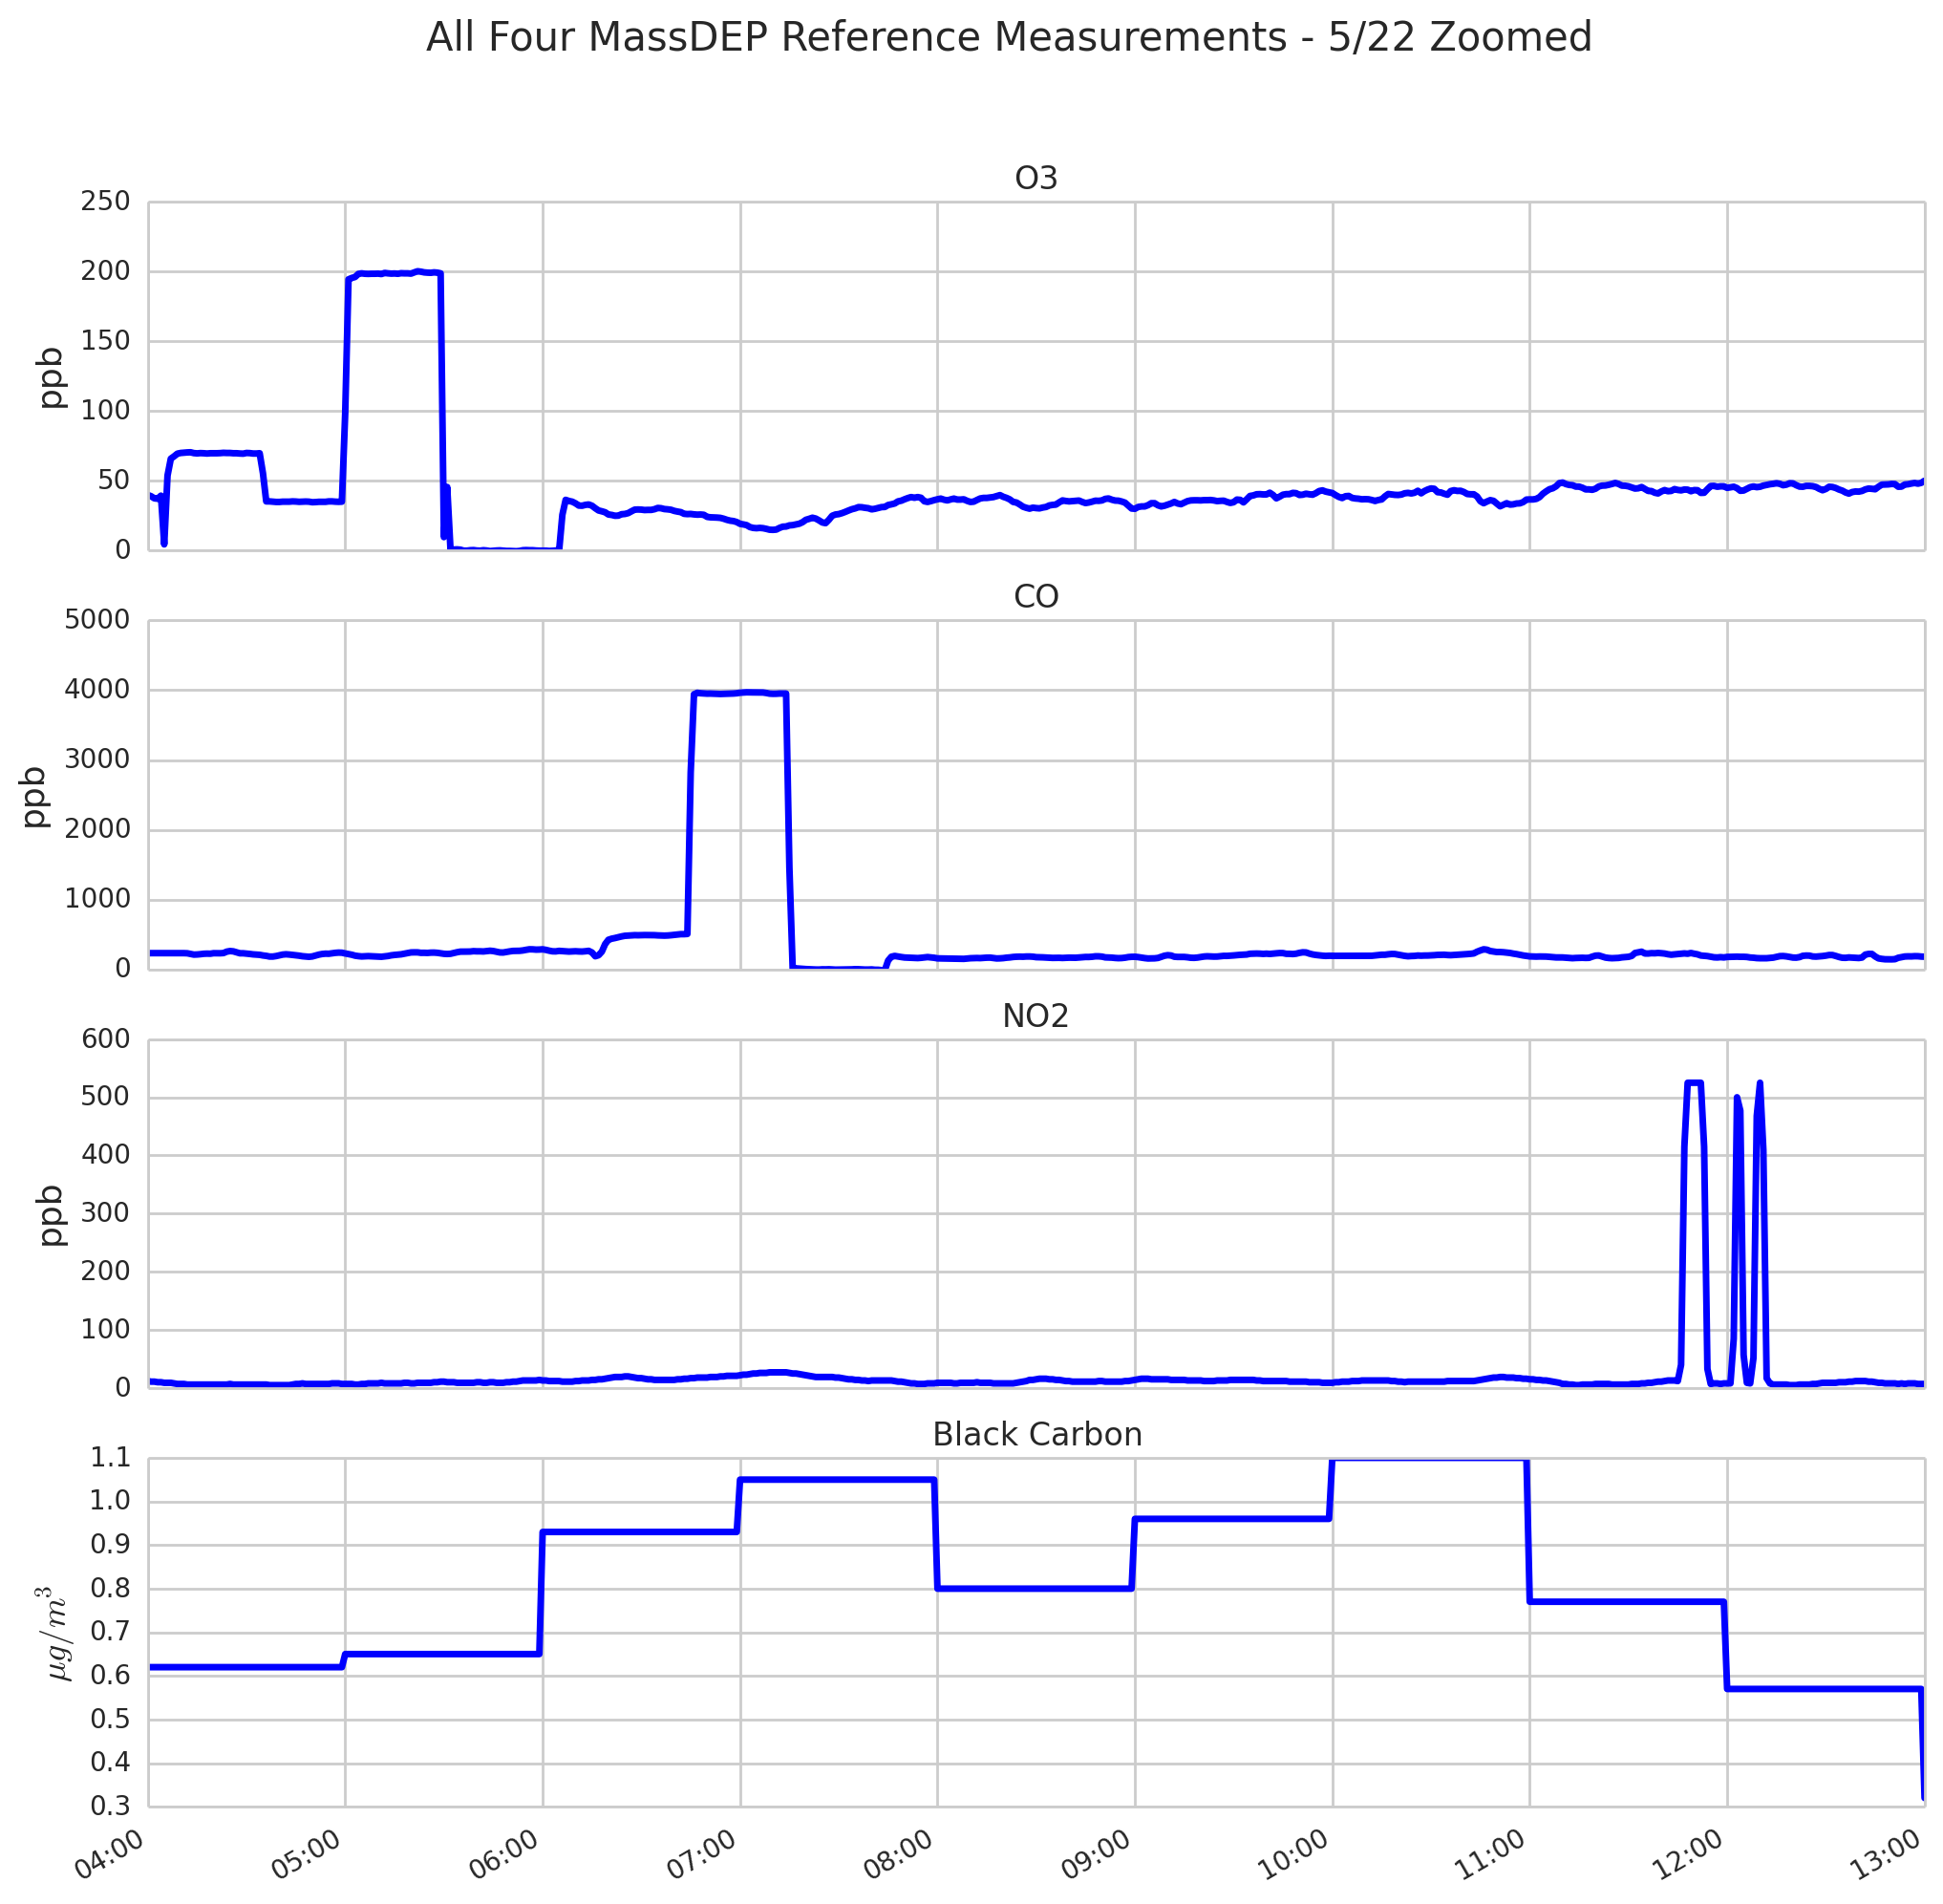
\includegraphics[width=\textwidth]{figs/epa_ref_measures_zoomed} 
             
 	 \caption{Two Example Transient Events Measured by Reference Sensors, 4/25 and 5/22}
  	\label{fig:epa_ref_measures_zoomed}
\end{marginfigure}


Generally, we see an inability to capture transient phenomena with the sensors we tested.  The cheaper NO2 and CO sensors on the SmartCitizen Kit showed no transient behavior.  The Alphasense NO2 also struggled to capture any transient events. The AlphaSense CO sensors reported a handful of small transients (0.5-1.5 ppm) that generally appear to match up with real transient events-- however, these transients were generally much smaller in magnitude than the actual, and most transients were still uncaptured.  The AlphaSense O3 sensor similarly captured a handful of transient events, with a closer match to the appropriate magnitude.  Unfortunately, it also missed about half of the transient events.

 These differences are interesting, and can potentially be explained in a few ways.  The SmartCitizen sensors (as expected) simply aren't of good enough quality to be sensitive and reactive enough to measure these differences.  They are speced for much higher concentrations at much lower resolutions.  The Alphasense sensors seem to have the ability to respond in the CO and O3 case.  These transients are actually quite long events, so there is no time-constant issue with the sensor physics.  Missed peaks and/or mis-measurments are likely due to airflow effects-- the reference sensor is actively pumping air through it, while the learnAir sensor is passively receiving airflow with some bias in its directionality.  The successful capture of a few transients suggest that the sensor physics are fundamentally up to the task.
 
NO2 transient events were much shorter duration events, and occur in the 0-400 ppb range.  The response time for a few of the narrower events could come into play, as the peaks clearly bump up against our 1-minute resolution (15 second rise time for 500 ppb); however, this is unlikely to be a primary factor, especially for some of the several minute transient events.  At the end of the day, these are slight changes in concentration (a few hundred ppb) occurring at much faster timescales than CO and O3, and it seems that the combination of these effects in conjunction with airflow made it impossible to detect.  It is worth further investigation to understand whether or not the sensor itself is capable of detecting these rapid events.
 

